\section{Le monde de GNU/Linux} \label{sec:GNU}

On entend souvent parler de Linux en tant que système d'exploitation, en opposition à Windows ou macOS. Il s'agit cependant d'un abus de langage. Le système est GNU/Linux, tandis que Linux est un noyau. Cette distinction fait toute son importance au regard de l'historique du système et de son placement sur le marché.

\subsection{L'ère UNIX - Début de l'informatique moderne}

\subsubsection{Généalogie des systèmes UNIX}
\textbf{UNIX est un des premiers systèmes d'exploitation}. Il est devenu public en 1971, mais sa conception et son développement ont commencé en 1969, notamment grâce à Ken Thompson et Dennis Ritchie, employés des laboratoires Bell. Le langage C a d'ailleurs été inventé pour écrire UNIX. Mais UNIX n'est pas le premier système d'exploitation : sa conception a été influencée par \textit{Multics} (issus de Bell Labs et du MIT), qui est également inspiré de \textit{CTSS} (développé par le MIT), dont la première version date de 1961, soit dix ans avant UNIX !

À sa sortie, le code source d'UNIX est alors privé. À partir de 1975, les universités peuvent acheter le code source pour l'utiliser, le modifier ou l'étudier. Les premiers systèmes basés sur UNIX apparaissent alors, comme l'illustre la figure \ref{fig:unix}.

\begin{figure}[hb!]
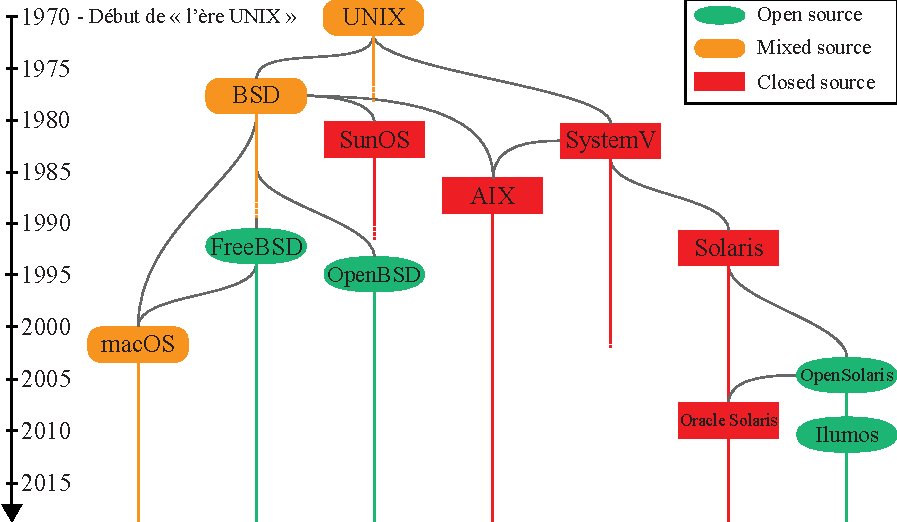
\includegraphics[width=\textwidth]{res/unix_genealogy.pdf}
\centering
\caption{Généalogie simplifiée des systèmes basés sur UNIX}
\label{fig:unix}
\end{figure}

La figure \ref{fig:unix} montre que de nombreux systèmes encore utilisés aujourd'hui sont basés sur UNIX ou ses descendants et qu'il existe de très forts liens entre les différents systèmes, qui s'inspirent et s'influencent mutuellement au cours du temps. Ceci peut souvent être mis en relation avec le fait que certains systèmes ont des sources fermées, ouvertes ou mixtes.

\newpage

\subsubsection{L'héritage d'UNIX}

Bien que UNIX ait été créé à la fin des années 60, on considère que l'ère UNIX ne commence qu'au 1\textsuperscript{er} janvier 1970. Cette date est un repère temporel important pour le monde de l'informatique. D'une part, il s'agit de la date symbolique à partir de laquelle sont apparus les prémices des systèmes actuels. D'autre part, elle est même utilisée comme base de mesure du temps : le nombre de secondes depuis le début de l'ère UNIX se nomme le \textit{timestamp}. Ceci témoigne de l'importance d'UNIX pour l'informatique actuelle.

Un autre aspect de l'importance d'UNIX réside dans les traces qu'il a laissé dans les systèmes d'exploitation, dont certains sont encore fortement utilisés aujourd'hui.

\paragraph{\href{https://www.openbsd.org}{OpenBSD} et \href{https://www.freebsd.org}{FreeBSD}}
Ces deux descendants directs de BSD, créés en 1996 et 1993, sont libres et \textit{open source}, avec un fort accent mis sur la fiabilité du système. OpenBSD est très centré sur la sécurité tandis que FreeBSD, de par sa volonté d'être un système multi-usages, est le système BSD le plus utilisé aujourd'hui. De nombreux éléments de FreeBSD sont d'ailleurs utilisés dans des systèmes dédiés à certains appareils tels que des consoles de jeux (Nintendo Switch, PlayStation 3 et 4\dots).

\paragraph{\href{https://www.ibm.com/power/operating-systems/aix}{AIX}}
Système développé par IBM en 1986, à partir de System V, et inspiré de BSD pour ses serveurs et \textit{mainframes}.

\paragraph{\href{https://www.apple.com/macos}{macOS}}
Anciennement nommé Mac OS X, ce système grand public bien connu et développé par Apple, est fourni gratuitement avec les ordinateurs de son concepteur depuis 2001. Auparavant, Apple distribuait son système propriétaire Macintosh OS depuis 1984. Ce double héritage, issu des différents acquisitions d'Apple, explique qu'une partie des sources sont ouvertes, mais pas libres, tandis que l'autre reste fermée.

\paragraph{\href{http://www.oracle.com/technetwork/server-storage/solaris}{Oracle Solaris}}
Suite à son rachat de Sun, développeur d'OpenSolaris, en 2009 Oracle a décidé de garder ses développements fermés pour créer son propre système propriétaire, dédiés pour ses serveurs.

\paragraph{\href{https://www.illumos.org}{Ilumos}}
Afin de conserver l'aspect open source d'OpenSolaris, la communauté a décidé, en 2010, de créer Ilumos, successeur libre d'OpenSolaris.

En revanche, on notera qu'\textbf{aucun lien hiérarchique entre UNIX et Linux ou GNU n'existe}. Linux et GNU ne sont donc pas des dérivés d'UNIX comme on peut le lire parfois. En revanche, il est indéniable qu'UNIX a influencé la naissance du projet GNU et la conception de Linux.

\newpage

\subsubsection{Le projet GNU}
Parallèlement, le \href{https://www.gnu.org/}{projet GNU} est initié en 1983 par Richard Stallman, qui souhaitait alors \textbf{créer un système d'exploitation complet et libre.} À l'époque, UNIX est assez répandu, mais reste propriétaire, son code source est n'est pas complètement ouvert, ni libre d'utilisation.
Le nom du projet GNU vient directement d'UNIX. Il s'agit d'un acronyme récursif : \textit{GNU's Not UNIX}. En utilisant directement le nom de son concurrent au sein de son projet, Stallman veut montrer la différence qui existe entre les deux systèmes malgré leur similitudes apparentes. C'est en effet en reprenant une partie des concepts d'UNIX, notamment en ce qui concerne son utilisation, que Stallman a construit GNU.

\subsubsection{Logiciel Libre}
Si Richard Stallman a posé ces bases techniques, c'est surtout par la notion de logiciel libre et sa volonté de le répandre et d'en faciliter l'accès qu'il a impacté l'informatique d'aujourd'hui. En effet, qu'il s'agisse de système d'exploitation entier ou de logiciels plus élémentaires, nombreux sont les projets ouverts et libres d'accès, d'utilisation, de partage et de modification.

C'est dans cette optique que Stallman a fondé la \href{https://www.fsf.org}{\textbf{Free Software Foundation}} en 1985, afin de pouvoir gérer les aspects administratifs, juridiques et organisationnels que demandaient le Projet GNU. Ainsi plusieurs licences sont issues de cette fondation, telles que la \href{https://www.gnu.org/licenses/quick-guide-gplv3.html}{\textit{General Public License} (GPL)} ou la \href{https://www.gnu.org/licenses/lgpl-3.0.en.html}{\textit{Lesser Public General License} (LGPL)}, qui sont devenues deux des licences de logiciel libre les plus utilisées. Si un code ou logiciel est distribué sous ces licences, alors toute personne peut est garantie des libertés suivantes : 
\begin{enumerate}
    \item la liberté d’exécuter le programme, pour tous les usages (y compris commercial),
    \item la liberté d’étudier le fonctionnement du programme et de l’adapter à ses besoins,
    \item la liberté de redistribuer des copies du programme,
    \item la liberté d’améliorer le programme et de distribuer ces améliorations au public, pour en faire profiter toute la communauté.
\end{enumerate}
Elle doit cependant toujours notifier les éventuelles modifications du code et laisser ce dernier accessible. De plus, la GPL impose de redistribuer toute modification avec la même licence. On dit alors que GPL est contaminante. Le terme \textit{copyleft}, popularisé par Stallman, est d'ailleurs un jeu de mot utilisé pour décrire la GPL, en opposition au \textit{copyright}.

Il existe de nombreuses autres licences de logiciels libres, créées par des universités ou des fondations impliquées dans le logiciel libre, qui respectent généralement ces libertés, mais précisent d'autres éléments. Le site TLDRLegal\footnote{\textit{Software Licenses in Plain English} - \href{https://tldrlegal.com}{https://tldrlegal.com}} permet de simplifier la compréhension de ces licences.
On pourra citer, notamment : 
\begin{itemize}
    \item \href{https://opensource.org/licenses/MIT}{Licence MIT} (du \textit{Massachusetts Institute of Technology}), qui n'est pas contaminante.
    \item Licences BSD (initiative de \textit{Berkeley Software Distribution}), proches de la licence MIT et établies pour le système BSD. Il en existe plusieurs variantes, toujours non contaminante.
    \item \href{https://www.apache.org/licenses}{Licence Apache}, initiée par la fondation Apache, n'est pas contaminante.
    \item \href{https://www.mozilla.org/en-US/MPL}{Licence Publique Mozilla}, initié par la fondation Mozilla, qui est n'est pas totalement contaminante, mais impose quelques restrictions.
    \item \href{https://creativecommons.org}{Licences \textit{Creative Commons}}, ensemble de licences prédéfinies et simples pour définir les libertés ou restrictions sur une œuvre.
\end{itemize} \vspace{\baselineskip}
\note{Note :} \textbf{Un logiciel peut être \textit{open-source} sans pour autant être considéré comme libre s'il est distribué sans licence ou qu'elle ne donne pas d'autorisations explicites.}

\newpage

\subsection{Généralités sur les systèmes d'exploitation}

\subsubsection{Système d'exploitation}

Un système d'exploitation (\textit{Operating System} ou \textit{OS} en anglais) est ensemble de logiciels permettant à un utilisateur d'exécuter des programmes sur un appareil en liant le matériel et les applications (voir figure \ref{fig:os}). Son rôle principal et de gérer, d'allouer et de protéger les ressources de l'appareil. C'est surtout le noyau (\textit{kernel}) du système qui se charge de ces tâches.

\subsubsection{Noyau}

Le noyau est véritablement le coeur du système d'exploitation. On peut regrouper ses missions en deux catégories : 
\begin{itemize}
    \item Faire l'interface entre le matériel et le logiciel,
    \item Gestion des ressources et des utilisateurs,
    \item Ordonnancement des tâches.
\end{itemize}

C'est donc lui qui permet d'orchestrer l'ensemble du matériel (RAM, clavier, disque dur...). Il permet ainsi à d'autres programmes d'accéder à ces composants et de les utiliser, par une interface unique, qui ne dépend pas du matériel. Les programmes sont ainsi libres d'utiliser le processeur pour effectuer des calculs, l'interface réseau pour contacter d'autres appareil du réseau voire accéder à Internet, ou encore utiliser le disque dur pour stocker des fichiers\dots Le noyau est généralement servi avec toute une série de programmes permettant à l'utilisateur de véritablement utiliser son ordinateur (interface graphique ou en ligne de commande, éditeurs de texte, utilitaires divers, etc.) formant ainsi un système complet et utilisable.

\begin{figure}[hb!]
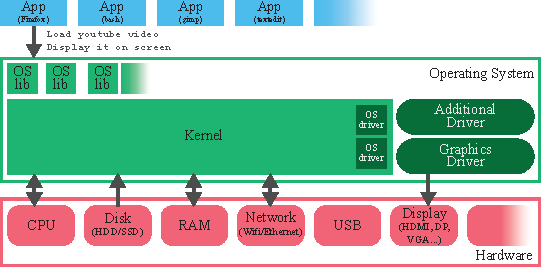
\includegraphics[width=\textwidth]{res/os_architecture.pdf}
\centering
\caption{Exemple de liens entre programmes, OS et matériel}
\label{fig:os}
\end{figure}

Il existe une multitude de systèmes d'exploitation et UNIX fut l'un d'entre eux. Par exemple, Windows, Android, iOS et macOS sont des systèmes d'exploitation. Tous les systèmes d'exploitation sont différents car ils ont été conçus avec des philosophies et contraintes matérielles différentes. C'est pour cela qu'il ne peuvent pas tous être installés sur les mêmes appareils et qu'ils s'utilisent différemment.

\newpage

\subsection{Les systèmes GNU/Linux} \vspace{-4mm}

\textbf{GNU/Linux est un ensemble de logiciels, issu du projet GNU, formant un système d'exploitation complet, libre et ouvert.} Linux, à lui seul, n'est pas un système d'exploitation à part entière puisqu'il s'agit d'un noyau. Le développement du noyau Linux a été initié par Linus Torvalds en 1991. Aujourd'hui, de très nombreux appareils (ordinateurs, serveurs, routeurs WiFi, consoles de jeu, téléphones\dots) utilisent un noyau Linux, ce qui rend les systèmes GNU/Linux majoritaires sur le marché des systèmes d'exploitation.

Ainsi, bien que UNIX soit un ancêtre commun à une multitude de systèmes d'exploitation encore utilisés aujourd'hui, \textbf{GNU/Linux en est totalement indépendant}. Richard Stallman et Linus Torvalds ont probablement été influencés par UNIX, mais GNU/Linux a été créé de zéro et n'est donc pas un dérivé d'UNIX, et ne figure pas sur la généalogie d'UNIX.

De plus, une autre fonctionnalité centrale aux distributions Linux est le système de paquets. Chaque programme est disponible sous forme de paquet, chaque paquet pouvant avoir des dépendances vers d'autres paquets. L'ensemble des paquets est disponible sur des serveurs proposant une interface commune à l'acquisition de programmes.

Il existe plusieurs systèmes utilisant un noyau Linux. La plupart sont regroupés sous le terme de \say{Distribution Linux}, puisque de nombreux logiciels sont distribués conjointement, en plus du noyau et des outils basiques formant le système GNU/Linux. Et, de la même manière que pour la généalogie d'UNIX, de très nombreuses distributions GNU/Linux existent et s'influencent les unes des autres, comme l'illustre la figure \ref{fig:distrib}.
\vspace{-2mm}
\begin{figure}[hb!]
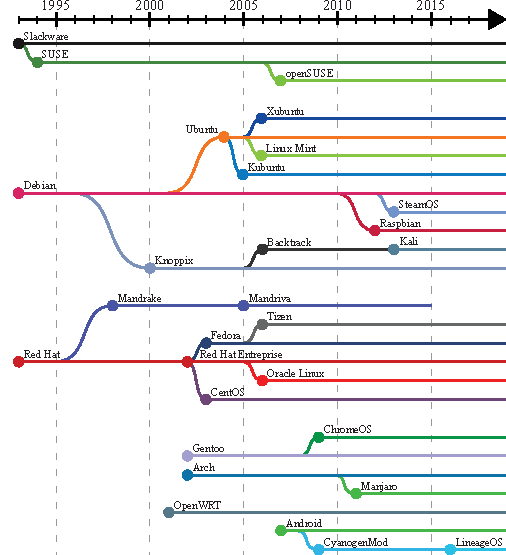
\includegraphics[width=0.70\textwidth]{res/linux_distrib_genealogy_links.pdf}
\centering
\vspace{-1mm}\caption{Généalogie simplifiée des principaux systèmes utilisant un noyau Linux}\label{fig:distrib}
\vspace{-\baselineskip}
\end{figure}

\newpage

\paragraph{Distributions basées sur Debian}

Il existe de nombreuses distributions basées sur \href{https://www.debian.org}{Debian}. Il s'agit d'une des distributions les plus anciennes, qui est la seule qui ne soit pas gérée par une entreprise. Debian met en avant la stabilité de son système, ce qui en a fait le favori des serveurs. Il existe plusieurs versions maintenue en parallèle, afin d'équilibrer entre stabilité et nouvelles fonctionnalités.

La variante la plus connue de Debian est \href{https://www.ubuntu.com}{Ubuntu}. Elle été créée afin de faciliter l'utilisation de Linux par le grand public. Elle dispose de plusieurs variantes (\href{https://kubuntu.org}{Kubuntu}, \href{https://xubuntu.org}{Xubuntu} ou \href{https://lubuntu.net/}{Lubuntu}) qui proposent un gestionnaire de bureau et des applications différentes, ainsi que d'autres variantes dédiées à des utilisations particulières. Il existe également des versions d'Ubuntu dédiée pour les téléphones : Ubuntu Touch. Le projet a été abandonné par Canonical mais repris par des développeurs indépendants.

\href{https://www.raspberrypi.org/downloads/raspbian/}{Raspbian} est une variante de Debian dédiée aux mini-ordinateurs Raspberry Pi. Elle est optimisée pour être exécutée sur ce système aux performances restreintes.

Les distributions basées sur Debian utilisent le système de paquets éponyme, avec les utilitaires \texttt{dpkg}\command{dpkg} pour gérer les paquets \texttt{.deb}, et \texttt{apt}\command{apt} pour gérer les dépendances et mises-à-jour de paquets.

\paragraph{Distributions basées sur Red Hat}

Red Hat (Entreprise Linux) est une des plus anciennes distribution, et est maintenue par l'entreprise du même nom.

Mandriva a été maintenue par une équipe française et se voulait simple d'utilisation. Elle est, depuis peu, reprise par la communauté sous le nom \href{https://www.openmandriva.org}{OpenMandriva}.

\href{https://www.centos.org}{CentOS} est le pendant libre de  \href{https://www.redhat.com/en/technologies/linux-platforms/enterprise-linux}{Red Hat Entreprise Linux} (RHEL). Dédiée aux serveurs, c'est une des distributions Linux les plus utilisées.

\href{https://getfedora.org/}{Fedora} est une autre distribution basée sur Red Hat. Elle propose des programmes libres et sous d'autres licences. Les nouveautés intégrées dans Fedora le sont a \textit{posteriori} dans Red Hat, ce qui en fait une des distributions les plus actualisées.
Les distributions basées sur Debian utilisent le système de paquets \textit{RPM} pour \textit{RPM Package Manager} (Anciennement \textit{Redhat Package Manager}. Le programme \texttt{yum}\command{yum} permet de gérer les paquets et leurs dépendances. Il a été remplacé par \texttt{dnf}\command{dnf} dans Fedora.

\paragraph{Distributions indépendantes}

\href{https://www.gentoo.org}{Gentoo} a été créé avec la conception que chaque programme doit être compilé avant d'être installé, ce qui permet de personnaliser l'installation et surtout d'optimiser la compilation pour le type d'ordinateur, permettant des performances légèrement meilleures.

\href{https://www.archlinux.org}{Arch Linux} est un système minimaliste, encourageant une forte implication de sa communauté. Ainsi, une installation Arch Linux est très légère car ne distribue que très peu de programmes supplémentaires. La prise en main s'en retrouve en revanche légèrement plus longue. Arch Linux dispose de son propre gestionnaire de paquets (\texttt{pacman}), et surtout une documentation extrêmement complète et détaillée. Elle dispose d'un pendant qui se veut facile à prendre en main : \href{https://manjaro.org}{Manjaro}.

\href{https://openwrt.org}{OpenWRT} est un système dédié pour les routeur WiFi et allégé de tous les composants non nécessaires pour cet usage particulier.

\href{https://www.android.com}{Android}, bien qu'il ne soit pas considéré à proprement parler comme une distribution Linux, est un système d'exploitation au noyau Linux, développé par Google. Il existe une variante principale, CyanogenMod, devenue \href{https://lineageos.org}{LineageOS}, qui est gérée par des développeurs indépendants.

\newpage

\subsection{Interfaces de contrôle}\vspace{-4mm}

Quel que soit le système d'exploitation, il dispose toujours d'une interface de contrôle (voir figure \ref{fig:interface}. Celle-ci peut être graphique ou en console. Dans le second cas, on parle de lignes de commandes, d'émulateur de terminal ou de terminal voire, en anglais, de \textit{CLI} pour \textit{Command Line Interface} et plus souvent de TTY (pour \textit{TeleTYpewriter}).
Le mode graphique varie grandement entre les systèmes d'exploitation et ce même pour des systèmes GNU/Linux. Il y cependant toujours un gestionnaire de bureau (\textit{desktop manager}) qui permet de gérer les fenêtres et programmes en cours d'exécution. Sous macOS, Windows et iOS, il n'existe qu'un seul gestionnaire de bureau possible.

En revanche, il existe une multitude de gestionnaire de bureau sous GNU/Linux, qui reposent sur différentes philosophies. C'est d'ailleurs souvent pour proposer un environnement graphique spécifique que des distributions Linux sont crées. Tous ces environnements sont cependant basés sur une couche logicielle standardisée, qui se nomme \href{https://www.x.org}{X}. Récemment, une nouvelle couche d'affichage graphique, \href{https://wayland.freedesktop.org}{Wayland}, a fait son apparition, mais son utilisation par les gestionnaire de bureau reste restreinte et difficile.

Généralement, il est possible d'utiliser une interface en ligne de commande à partir d'une interface graphique et cela offre plusieurs avantages. Premièrement, on peut bénéficier des fonctionnalités du mode graphique telles que la souris ou le \textit{multitasking} (utilisation de plusieurs applications simultanément) via l'utilisation de fenêtres pour les programmes. Mais lorsqu'aucun gestionnaire de bureau n'est installé, la ligne de commande pure (sans fenêtre, ni souris, uniquement du texte) est incontournable.

Enfin, l'interface en ligne de commande permet souvent un contrôle rapide et fin de ce que l'on souhaite faire, puisqu'aucune surcouche ne masque ce qui est réellement exécuté. L'interface en ligne de commande permet donc de mieux comprendre ce que l'on fait, ainsi que le fonctionnement du système. Elle nécessite en revanche un apprentissage plus long et moins instinctif qu'une interface graphique interactive.

\begin{figure}[hb!]
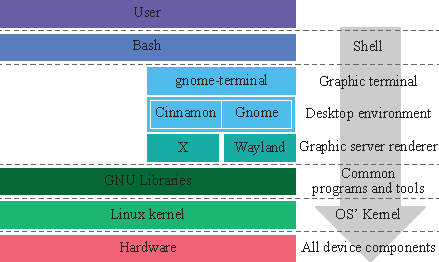
\includegraphics[width=0.78\textwidth]{res/linux_control_interface.pdf}
\centering
\caption{Schéma des couches de contrôle d'un système GNU/Linux}
\label{fig:interface}
\end{figure} \vspace{-2mm}

\note{Note :} Dans la figure \ref{fig:interface}, on peut remarquer que la couche graphique est totalement optionnelle pour utiliser le système. De plus, un seul serveur graphique peut être utilisé à la fois. De même pour les environnements de bureau, qui restent cependant indépendants du serveur graphique.